%!TEX root = ../dissertation.tex

\chapter{Introduction}
\label{chapter:introduction}

\section{Context}
Nowadays the demand for better mobile devices is higher than ever. Mobile phones are an indispensable gadget in today's society. Increasingly demanding application and connectivity requirements bring the need for devices with more capabilities, \textit{e.g.} battery life, memory, persistent storage, Internet access speeds, \textit{etc.} With this evolution of equipment, inevitably, comes an evolution of communication technologies.

Mobile phones, usually communicate between themselves in different ways: via mobile cellular networks, via Internet access, via Bluetooth, \textit{etc.} New communication technologies are appearing at a fast pace and the possibilities for using them to provide new services for the users are endless.

The main communication methods use a limited number of central points, that coordinate the communication process between devices, acting as mediators in the communication channel. However, from this dependence, a question arises: if there is a limited number of central points what happens if a partial or total failure from their part occurs. This question has an answer in device to device communications.

There are many devices available, usually more than one per person, see \cite{dpp}, making the creation of an ad hoc network a big possibility to overcome possible failures with central points or even if one is not within reach of any central point. Despite that, this answer is not a substitute to the existing communication methods. It aims to add more range and robustness to the network and possibly reduce the workload of the infrastructured network, which has a limited capacity.

Due to the reasons just stated, ad hoc communication between devices has been lately a hot topic, with several applications being currently offered to mobile users \textit{e.g.} FireChat and Ueppa!, see Section \ref{sec:apps}. This thesis offers a framework to create applications of this nature. To realise this framework a new application of this kind was implemented which allows users to access web pages using ad hoc links when they are not within range of an access point or base station. 

\section{Problem Statement}

Given the context above, the main question is: where can the creation of an ad hoc network be of use to the everyday tasks people perform on their mobile devices. There are many answers to this question, thus the difficulty of choosing a relevant topic. Much of the work currently being done focus on chat applications, where messages are transmitted via an ad hoc network. Bearing this in mind, this thesis takes a further step and creates a framework to form an ad hoc network capable of transmitting packets between devices.

\begin{figure}[ht]
	\noindent\makebox[\textwidth]
	{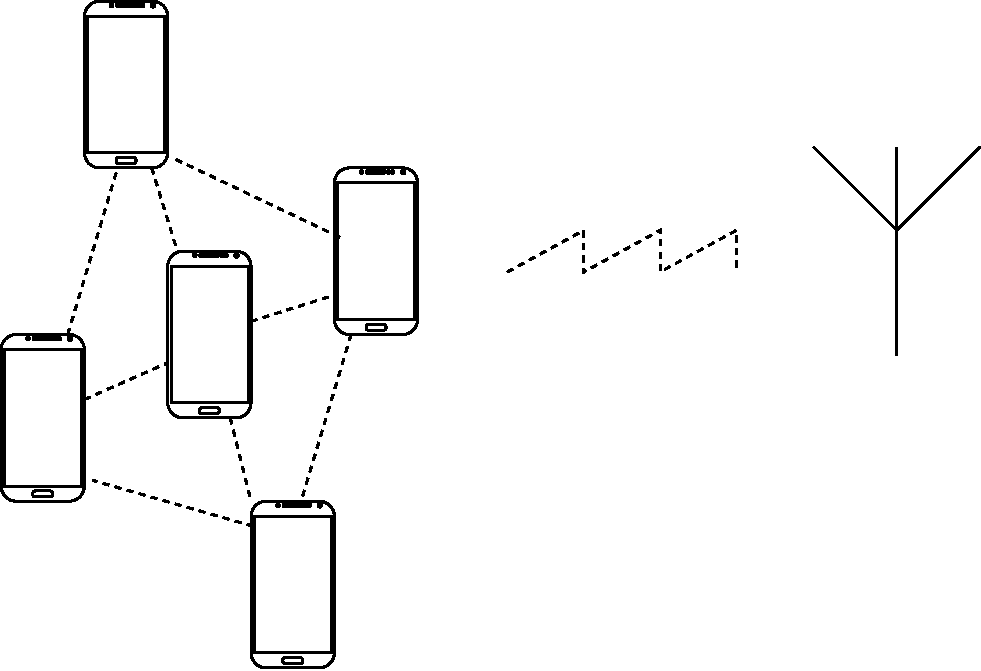
\includegraphics[width=0.8\textwidth]{images/context.pdf}}
	\caption{\label{fig:context} Example of a created ad hoc network}
\end{figure}

A solution is proposed to solve the inability of devices to access web pages, through a peer-to-peer application, even where there is the possibility of indirect Internet access, via communication with other devices and not directly with the infrastructure. The Android hotspot is an existing service that allows devices to share their Internet with the surrounding peers. However, this only works if a device is within immediate range of the hotspotting device, reducing the size and reach of the created network. In the solution proposed in this thesis, the devices are able to reach the Internet by sending their requests to their immediate peers, who will forward them to their neighbors until the destination is reached, travelling more than one hop\footnote{One hop is the distance of the communication between a device and its immediate peers. Each time the message travels between a device and its peers a hop is added to the message path.}, see the example of Figure \ref{fig:context}.

It is important to note that this work does not have the purpose of replacing the existing communication infrastructure, but is, in fact, trying to complement it.

\section{Objectives}
\label{sec:objectives}

This thesis will pursue two main objectives:

\begin{enumerate}
	\item 
	Developing a framework to create of a decentralized ad hoc network, where packets are transmitted between devices. Proving that, with the current unmodified Android versions and the Bluetooth technology, the creation of a network of that nature is feasible.
	
	To materialize the framework an application that implements this framework and exchanges web pages between devices is created. The application will create a solid ad hoc network. After the creation is complete the application will provide the logic to correctly manage the web pages request throughout the network, as well as their correct delivery. This application will then be submitted to a series of tests to comprehend where it is more vulnerable and where it is more robust.
	
	\item 
	The second objective will be to assess the advantages of migrating this application from Bluetooth to Wi-Fi Direct and what changes need to be made to the current Android versions to accommodate this migration. The advantages and disadvantages of Wi-Fi Direct in comparison to Bluetooth will be compared in the scope of the created framework. Conclusions will be drawn from a series of tests to compare both technologies. Also, a description of the obstacles, present in the current Android devices, preventing the development of this application using Wi-Fi Direct instead will be presented.
	
\end{enumerate}

This thesis will not provide a market product, thus it disregards some aspects of what would be to expect from a full consumer ready application. Security is not developed in this solution, although some ideas are given on how it can be provided.

\section{Contributions}

As mentioned before the created framework has a huge amount of possibilities. The purpose of this thesis is not to limit these possibilities to the transfer of web pages. It is to provide a simple to use developer kit that can be extended easily to exchange any message format, from web pages to beacon messages.

This is an open source framework and it is hosted in a GitHub repository\footnote{To download the code of the application clone the following repository: \url{https://github.com/Falcato/ThesisApp.git}.}. In here the full application code will be presented with the necessary comments to complement the description made in Chapter \ref{chapter:work}. By using the provided mechanisms developers can made the necessary modifications to the code in order to achieve different goals, \textit{e.g.} the creation of a peer-to-peer chat application.

Also, since the transfer of web pages is a complicated process and not much information is available on it, this application has a double usefulness, since it also demonstrates how to exchanges large files between devices.

A set of study tests on the advantages and disadvantages of Bluetooth and Wi-Fi Direct is presented in an easy and succinct fashion. Finally, several study tests on a not so common environment, a Bluetooth peer-to-peer application, are provided, revealing this technology's performance in an Android application.

\section{Structure of the Thesis}

The rest of this thesis is organized as follows:

\begin{itemize}
	
	\item Chapter \ref{chapter:soa} will begin with a theoretical introduction of the different wireless communication technologies, analysing their features, advantages and disadvantages. This aims to provide the needed background to understand the technologies used in this thesis and the choices made along its developments. There will be an analysis on the Android's implementation of Bluetooth and Wi-Fi Direct, as well as some of the possibilities it may present, such as ad hoc networking and multi-hop routing. Finally, an overview of some ad hoc networking applications in Android will be given, describing their features and technologies used.
	
	\item Chapter \ref{chapter:work} will contain the implementation of both framework and application. It will begin by a description of the steps taken to decide important parts of the framework, such as technologies and routing protocols used. The implemented network creation and communication protocols are explained, providing a better understanding of the framework. Lastly, the materialization of the framework, the peer-to-peer application to exchange web page is described, along with its features and overall packet exchanges.
	
	\item Chapter \ref{chapter:tests} will provide a theoretical and empiric evaluation of Bluetooth and Wi-Fi Direct, assessing how both technologies fare in certain aspects, useful for the proposed framework. Furthermore, several experiments will be performed on the developed application, in order to point its overall performance, strong and weak points.
	
	\item Chapter \ref{chapter:conclusion} will discuss the possible future work to be developed in the proposed framework and application. A final summary of what was developed and accomplish in this thesis will be presented.
	
\end{itemize}








